% one-figure manuscript written by fig_qc.py --tek-sekil-tex (trap T29)
\begin{figure*}[!t]
\centering
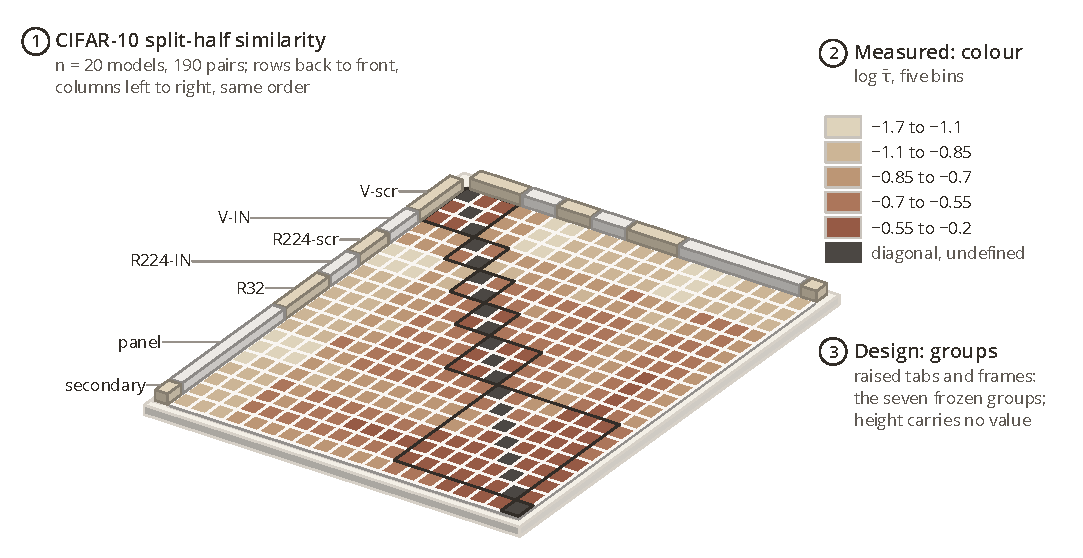
\includegraphics{pv_c_relief}
\caption{\textbf{CIFAR-10 pairwise similarity on a plinth.} The 20×20 split-half log τ̄ matrix lies flat in frozen group order (1); cell colour is one of five pooled quintile bins (2); raised edge tabs and frames mark the seven frozen groups (3). No height carries a measured value; the dark diagonal is undefined.}
\label{fig:pv_c_relief}
\end{figure*}
